
\section{Three transverse foliations determine the zoom}\label{sec:zoom}

Exact preservation of three transverse families of parallel lines is
an affine rigidity phenomenon; see Artstein-Avidan and Slomka
\cite{ArtsteinSlomka2017}. We need a compactness statement that also
rules out collapse before a limit map has been obtained.
The following elementary lemma prevents a change of coordinates from
collapsing at the scale under consideration.  Its monotonicity hypothesis
is imposed before any fixed linear change of the target coordinates.
For a vector $v$, write $[v]$ for its unoriented line through the origin.

\begin{lemma}[Three-foliation compactness]\label{lem:three-foliation}
Let $\Omega_j\subset\mathbb R^2$ be open sets containing every compact
subset of $\mathbb R^2$ for all sufficiently large $j$.  Let
$F_j:\mathbb R^2\longrightarrow\Omega_j$ be homeomorphisms.  Put
$v_1=(1,0)$, $v_2=(0,1)$ and $v_3=(1,1)$.  Suppose the following hold.
\begin{enumerate}
\item There is a fixed invertible matrix $P$ such that each coordinate
of $P F_j$ is monotone on each line parallel to $v_i$.  For each $i$,
the two monotonicity signs are independent of the line and of $j$.
\item Along every subsequence, if $x_j,y_j$ lie on one line parallel to $v_i$ and
$F_j(x_j)\to a$, $F_j(y_j)\to b$, then $b-a\in\mathbb R v_i$.
The points and their common line may depend on $j$.
\item $F_j(0)=0$ and $|F_j(v_1)|=1$.
\end{enumerate}
After passage to a subsequence there is $\sigma\in\{-1,1\}$ such that
$F_j\to \sigma\operatorname{id}$ uniformly on compact sets.  The inverse
maps converge to $\sigma\operatorname{id}$ uniformly on compact sets as
well.
\end{lemma}

\begin{proof}
We first control images of entire lines and intersections between
families. Those intersections then determine the map on rational grids; coordinate
monotonicity will extend this control to compact sets. The final step
will control the inverse maps.

To begin, we show that entire line images, including lines with moving base
points, converge to the prescribed target lines.  Fix a family $i$ and
points $x_j$ with $a_j=F_j(x_j)\to a$.  Orient the source lines in the
direction $v_i$.  Their forward target displacements belong to a fixed
closed pointed cone $Q_i$, the inverse under $P$ of the signed coordinate
quadrant specified by the first hypothesis.  Choose a linear functional
$\ell_i$ strictly positive on $Q_i\setminus\{0\}$.  There is $M_i<\infty$
such that
\[
 |q|\le M_i\ell_i(q)\qquad(q\in Q_i).
\]
Consequently $s=\ell_i(F_j(x)-a_j)$ is a strictly increasing continuous
parameter on the image of this oriented source line: injectivity rules
out equality at two points.  In this parameter its image $\gamma_j$ is
$M_i$-Lipschitz.

The parameter intervals exhaust $\mathbb R$.  Indeed, for any fixed
$R$, a ball containing all points at distance at most $M_iR+1$ from
$a_j$ lies in $\Omega_j$ for large $j$.  The preimage of its closure is
compact, so each source ray eventually leaves that ball.  The cone
inequality forces its parameter to exceed $R$ in the positive direction
or to be less than $-R$ in the negative direction.  This proves the
claim without any control of the Euclidean locations $x_j$.

At parameter $s=1$, a convergent subsequence gives a nonzero vector
in $Q_i\cap\mathbb R v_i$: its $\ell_i$ value is one.  Thus this
intersection contains a ray, and pointedness makes the ray unique.
Compactness of equi-Lipschitz curves and the second hypothesis now imply
\[
 \gamma_j(s)\longrightarrow a+s\frac{d_i}{\ell_i(d_i)}
 \quad\hbox{locally uniformly in }s,
\]
where $d_i$ is the unit vector on $\mathbb R v_i$ belonging to $Q_i$.
There is exactly one such ray; $\ell_i(d_i)>0$.  The formula also shows
that the limit is unique, so no additional subsequence is needed for
this assertion.  In particular the line image traces the entire
limiting line in both directions.

It follows that intersections of two different families converge.
More precisely, let two source lines of types $i\ne k$ have base
images tending to $a$ and $b$.  The two limiting lines intersect at a
unique point $c$.  In a small parallelogram around $c$ with sides
parallel to these limiting directions, the preceding parameterized
convergence produces arcs close to the two transverse diameters and
joining their respective opposite sides.  They intersect by planar
separation, in the opposite-sides form of
\cite[Lemma~2.11]{PascolettiZanolin2010}.  The source lines have exactly one intersection, and their
images do also because $F_j$ is a homeomorphism.  Hence this unique
intersection is inside every sufficiently small such parallelogram
eventually, proving convergence to $c$.  The argument allows $a=b$;
transversality concerns the two line types, not the two base points.

We have controlled intersections even when their base points move.
We next use those intersections to determine the scale at every rational
point, starting from the normalized pair $0,v_1$.

Pass to a subsequence so $F_j(v_1)$ converges.  Its limit is
$\sigma v_1$ with $\sigma=\pm1$ by the second and third hypotheses.
Starting with $0,v_1$, intersections of horizontal, vertical and
slope-one lines generate the integer lattice.  For example the
diagonal through $0$ meets the vertical through $v_1$ at $(1,1)$;
its horizontal meets the vertical through $0$ at $(0,1)$.
The diagonal through $v_1$ meets that vertical at $(0,-1)$.
These operations and their reverses give each integer step and then
every lattice intersection; Figure~\ref{fig:three-foliation-grid} shows
the first steps. Intersection convergence proves
$F_j(z)\to\sigma z$ at all integer lattice points.

\begin{figure}[htbp]
\centering
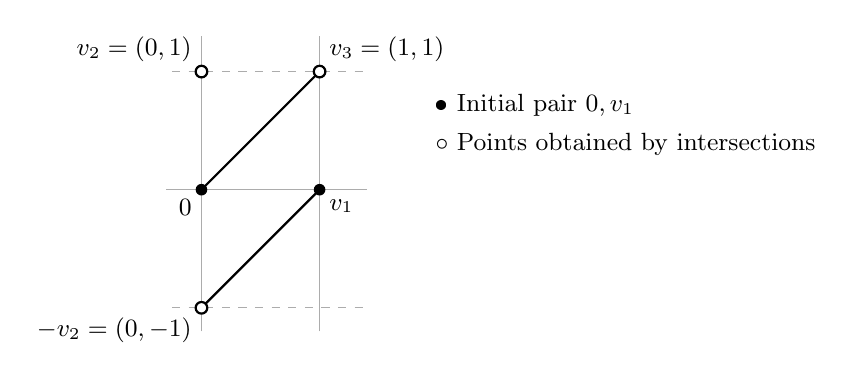
\begin{tikzpicture}[x=1.5cm,y=1.5cm,font=\small]
  \draw[gray!65] (-.3,0)--(1.4,0);
  \draw[gray!65] (0,-1.2)--(0,1.3);
  \draw[gray!65] (1,-1.2)--(1,1.3);
  \draw[gray!65,dashed] (-.25,1)--(1.4,1);
  \draw[gray!65,dashed] (-.25,-1)--(1.4,-1);
  \draw[thick] (0,0)--(1,1);
  \draw[thick] (0,-1)--(1,0);
  \fill (0,0) circle (2.1pt);
  \fill (1,0) circle (2.1pt);
  \draw[fill=white,thick] (1,1) circle (2.1pt);
  \draw[fill=white,thick] (0,1) circle (2.1pt);
  \draw[fill=white,thick] (0,-1) circle (2.1pt);
  \node[below left] at (0,0) {$0$};
  \node[below right] at (1,0) {$v_1$};
  \node[above right] at (1,1) {$v_3=(1,1)$};
  \node[above left] at (0,1) {$v_2=(0,1)$};
  \node[below left] at (0,-1) {$-v_2=(0,-1)$};
  \node[align=left,anchor=west] at (1.9,.55)
       {\textbullet\ Initial pair $0,v_1$\\[3pt]
        $\circ$\ Points obtained by intersections};
\end{tikzpicture}
\caption{The source-plane intersection construction using horizontal,
vertical and slope-one lines. The diagonal through $0$ meets the vertical
through $v_1$ at $v_3$; its horizontal gives $v_2$. The diagonal through
$v_1$ meets the vertical through $0$ at $-v_2$. Convergence of the image
intersections is proved in the text.}
\label{fig:three-foliation-grid}
\end{figure}

Fix $m\ge1$.  By the original two coordinate monotonicities,
$P F_j(v_1/m)$ is in the coordinate rectangle with vertices $0$ and
$P F_j(v_1)$, so it is bounded.  Every subsequential limit is $b v_1$
by the second hypothesis.  Apply the same finite intersection
construction with seed $v_1/m$ in place of $v_1$.  It constructs
$v_1$ after $m$ additions, and intersection convergence shows that
its limiting image is $mbv_1$.  Thus $mb=\sigma$.
This argument is valid even if one initially supposes $b=0$, since
every intersection is between two different line types.  Therefore
$F_j(v_1/m)\to\sigma v_1/m$ without a noncollapse assumption.
Repeating the grid construction proves convergence on
$(m^{-1}\mathbb Z)^2$, and hence at every rational point.

Finally squeeze each coordinate of $P F_j$ between the appropriate
corners of a rational grid cell.  The signs can differ between the
two coordinates and the two source axes; choose the lower and upper
corners for each coordinate separately.  The limiting corner values
are those of $\sigma P x$, whose oscillation on a cell is bounded by
a constant times its mesh.  A finite grid covering a compact set
therefore proves uniform convergence there.  This uses monotonicity
of $P F_j$, not an unjustified monotonicity of $F_j$.

For inverse convergence, choose a circle sufficiently large to contain
a given compact target set with positive margin.  Uniform convergence
on that circle and the Jordan curve theorem
(see \cite{Siebenmann2005}) show that its image
encloses the target set for large $j$; this image bounds the image of
the source disk.  The inverse images of the target set are thus
uniformly bounded.  Uniform convergence of $F_j$ on that disk gives
uniform convergence of the inverses.
\end{proof}

\subsection{Application to the rank coordinates}

Fix a rank point $p$ where all functions $f_C$ are differentiable and
where the directional conclusion already proved holds.  Choose three
times $\tau_1,\tau_2,\tau_3$ whose allowed direction sets are singletons
and are pairwise projectively distinct.  Let their unit directions
be $d_1,d_2,d_3$.  Fix an invertible matrix $B$ carrying
$[d_1],[d_2],[d_3]$ to $[v_1],[v_2],[v_3]$.

Consider any radii $h_j\downarrow0$ and indices tending sufficiently
fast that, on every bounded set of $w$ and for every fixed $C$,
\begin{equation}\label{eq:zoom-expansion}
 r_{C,j}(p+h_jw)=f_C(p)+h_j\nabla f_C(p)\cdot w+o(h_j).
\end{equation}
Here $r_{C,j}$ denotes the $C$ coordinate as a function of the pair
of rank coordinates, and the error is uniform on the bounded set.
This diagonal condition follows from monotone squeezing at continuity
points and differentiability at $p$.  It asserts no uniform rate in
the configuration index.

Normalize the original Euclidean plane linearly so its three
$\tau_i$ directions become $[v_i]$, translate the preimage of $p$ to
$0$, and scale the whole plane so the image of $v_1$ under the rank
zoom $B(r-p)/h_j$ has norm one.  Such a scale exists: on the chosen
horizontal ray the rank zoom is continuous, starts at zero, and exits
every fixed ball contained in its expanding target domain.
Let $F_j$ be this map from the normalized Euclidean plane to rank
zoom coordinates.

The first hypothesis of Lemma~\ref{lem:three-foliation} holds with
$P=B^{-1}$, by the two original rank-coordinate monotonicities;
passing to a subsequence fixes any orientation signs.  Its second
hypothesis follows from \eqref{eq:zoom-expansion}: every bounded limiting displacement on
a $\tau_i$ line satisfies all its directional sign constraints, so
it is parallel to $B d_i$, whether or not its base point moves.
The target domains exhaust the plane since $p$ is interior to the
rank square.  The lemma therefore applies.  In this normalization
the zoom and its inverse converge locally uniformly to a nonsingular
linear map; with the stated choice they converge to $\sigma I$.

We must compare this point-dependent normalization with the common
normalization based on three fixed times $t_1<t_2<t_3$: in each
configuration a linear map sends their projective directions to a
prescribed fixed triple.  Let $L_j$ map the open rank square to this
common normalized Euclidean plane, by inverting the rank map and
applying that linear map.  At our point
their allowed direction sets $D_p(t_i)$ are compact and pairwise
disjoint.  Let $\xi_{i,j}$ be their projective directions in the
$\tau$-normalized Euclidean plane.  After any further subsequence
these directions have limits.  Testing a unit segment through the
origin in direction $\xi_{i,j}$ in the uniformly convergent maps
shows that its limiting image direction, after undoing $B$, belongs
to the projectivization of $D_p(t_i)$.  Equivalently, orient the
tested segment in the original forward direction to obtain an
oriented limit in $D_p(t_i)$.  Thus the limiting directions lie in three fixed,
pairwise disjoint compact subsets of the projective line.  Their
separation is bounded below by a positive number depending only
on $p$ and the two fixed triples, independently of this zoom sequence.

Let $A_j$ convert the $\tau$ normalization to the common normalization,
which sends the $t_i$ directions to a prescribed fixed triple.
These matrices have bounded condition number.  Indeed normalize
$\|A_j\|=1$ and suppose a limit were singular.  At most one of three
separated limiting input directions could be its kernel, so two
others would have the same limiting output direction.  This
contradicts the two corresponding distinct fixed output directions.
Compactness gives a bound depending only on the separation and the
fixed target triple.

It follows that for every diagonal satisfying \eqref{eq:zoom-expansion}, after translations,
positive scalar rescalings and a subsequence, the common-coordinate
maps
\[
 w\longmapsto L_j(p+h_jw)-L_j(p)
\]
converge locally uniformly to an invertible linear map of condition
number at most $K_p<\infty$.  Indeed the normalized limit is
$\sigma A B$, with $A$ a nonsingular scalar-normalized limit of
$A_j$; the bound includes the fixed condition number of $B$.

Define
\[
 U_j(p,h)=\max_{|u-p|=h}|L_j(u)-L_j(p)|,
 \qquad
 V_j(p,h)=\min_{|u-p|=h}|L_j(u)-L_j(p)|.
\]
Choose $C_p>K_p$.  For each integer $T\ge2$, there exists
$h_{p,T}>0$ such that for every fixed $0<h<h_{p,T}$ and every
sufficiently late configuration $j$,
\begin{equation}\label{eq:radial-comparison}
 V_j(p,h/T)\ge\frac{U_j(p,h)}{C_p T},
 \qquad
 U_j(p,h/T)\le\frac{C_p V_j(p,h)}{T}.
\end{equation}
If either eventual comparison failed for arbitrarily small fixed
radii, choose radii tending to zero and failing indices arbitrarily
late, late enough also to satisfy \eqref{eq:zoom-expansion}.  Pass to the just-established
linear limit.  On the two circles its radial maxima and minima have
ratios $T\kappa$ and $\kappa/T$, respectively, with
$\kappa\le K_p<C_p$, contradicting failure.  This proves \eqref{eq:radial-comparison} in the
order stated: first the fixed radius, then the configuration index.
